\documentclass[prl,preprintnumbers,twocolumn,eqsecnum,floatfix,a4paper,nofootinbib,superscriptaddress]{revtex4}
\usepackage{color}
\usepackage{calc}
\usepackage{amsmath,amssymb,graphicx}
\usepackage{amssymb,amsmath}
\usepackage{bm}
\usepackage{microtype}
\usepackage{booktabs}
\usepackage{times}
\usepackage[varg]{txfonts}
\usepackage[colorlinks, pdfborder={0 0 0}]{hyperref}
\usepackage[utf8]{inputenc}
\definecolor{LinkColor}{rgb}{0.75, 0, 0}
\definecolor{CiteColor}{rgb}{0, 0.5, 0.5}
\definecolor{UrlColor}{rgb}{0, 0, 0.75}
\hypersetup{linkcolor=LinkColor}
\hypersetup{citecolor=CiteColor}
\hypersetup{urlcolor=UrlColor}
\maxdeadcycles=1000
\allowdisplaybreaks
\textwidth 7 in
\hoffset -0.1in
\textheight 10in
\DeclareFontFamily{OT1}{pzc}{}
\DeclareFontShape{OT1}{pzc}{m}{it}{<-> s * [1.10] pzcmi7t}{}
\DeclareMathAlphabet{\mathpzc}{OT1}{pzc}{m}{it}

\newcommand{\red}[1]{\textcolor{red}{#1}}
\newcommand{\comment}[1]{\textcolor{blue}{\textit{#1}}}
\newcommand{\ajith}[1]{\textcolor{red}{\textit{Ajith:#1}}}
\newcommand{\checkthis}{\textcolor{magenta}{(CHECKTHIS)}}
\newcommand{\vijay}[1]{\textcolor{cyan}{Vijay: #1}}
\newcommand{\io}{\iota}
\newcommand{\p}{\phi}
\newcommand{\vp}{\varphi}

\newcommand{\h}{\mathpzc{h}}
\newcommand{\Hhat}{\hat{\mathpzc{H}}}
\newcommand{\B}{\mathpzc{B}}
\newcommand{\hlm}{\mathpzc{h}_{\ell m}}
\newcommand{\xilm}{\xi_{\ell m}}
\newcommand{\Ylm}{{Y}^{-2}_{\ell m}}
\newcommand{\Y}{{Y}^{-2}}
\newcommand{\hc}{h_\times}
\newcommand{\hp}{h_+}
\newcommand{\Fc}{F_\times}
\newcommand{\Fp}{F_+}
\newcommand{\Mf}{M_f}
\newcommand{\cA}{\mathpzc{A}}
\newcommand{\lm}{_{\ell m}}
\newcommand{\deff}{d_\mathrm{eff}}
\newcommand{\rmi}{\mathrm{i}}
\newcommand{\blambda}{\bm{\lambda}}
\newcommand{\btheta}{\bm{\theta}}
\newcommand{\bxi}{\bm{\xi}}
\newcommand{\etal}{\emph{et al}}
\newcommand{\n}{\mathbf{n}}

\begin{document}

%\title{A consistency test of general relativity using different multipoles of \\gravitational radiation from binary black holes}
\title{Binary black hole spectroscopy: A ``no-hair'' theorem test for binary black holes}

\author{Siddharth Dhanpal}
\affiliation{International Centre for Theoretical Sciences, Tata Institute of Fundamental Research, Bangalore 560012, India}
\author{Abhirup Ghosh}
\author{Ajit Kumar Mehta}
\affiliation{International Centre for Theoretical Sciences, Tata Institute of Fundamental Research, Bangalore 560012, India}
\author{Parameswaran~Ajith}
\affiliation{International Centre for Theoretical Sciences, Tata Institute of Fundamental Research, Bangalore 560012, India}
\affiliation{Canadian Institute for Advanced Research, CIFAR Azrieli Global Scholar, MaRS Centre, West Tower, 661 University Ave., Suite 505, Toronto, ON M5G 1M1, Canada}
\author{B.~S.~Sathyaprakash}
\affiliation{The Pennsylvania State University, University Park, PA 16802, USA}

\begin{abstract}
One of the consequences of the black-hole ``no-hair'' theorem in General Relativity (GR) is that gravitational radiation (\emph{quasi-normal modes}) from a perturbed Kerr black hole is uniquely determined by its mass and spin. Thus, different quasi-normal modes have to be consistent with the same value of the mass and spin. Similarly, the gravitational radiation from a coalescing binary black hole system is uniquely determined by a small number of parameters (masses and spins of the black holes and the orbital eccentricity). Thus, consistency between different spherical harmonic modes of the radiation is a powerful test of the consistency of the signal with a binary black hole system in GR. We formulate such a test of GR, develop a Bayesian implementation, demonstrates its performance on simulated data and investigates the possibility of performing such a test using upcoming GW observations. 
\end{abstract}
\preprint{LIGO-P1800056-v1}
\maketitle
%%%%%%%%%%%%%%%%%%%%%%%%%%%%%%%%%%%%%%%%%%%%%%%%%%%%%%%%%%%%%%%%%%%%%%%%%%%%%%%%%%%%%%%%%%%%%%%%%%%%%%%%%%%%%%%%%%%%%%%%%%%%%%%%%%%%%%%%%%%%%%%`
\paragraph{Introduction:---}


One of the remarkable predictions of general relativity (GR) is that a stationary black hole can be fully described by a small number of parameters --- its mass, spin angular momentum and electric charge~\cite{Israel:1967,Israel:1968,Carter:1978}. As a consequence of this ``no-hair'' theorem, frequencies of the gravitational radiation (\emph{quasi-normal modes}~\cite{Vishveshwara:1970zz,Press:1971wr,Chandrasekhar:1975zza}) from a perturbed black hole is fully determined by these parameters. Astrophysical black holes are expected to possess negligible electric charge; hence, different quasi-normal modes have to be consistent with the same value of the mass and spin. Thus, the consistency between multiple quasi-normal modes provides a test of the ``no-hair'' theorem for stationary, isolated black holes~\cite{Dreyer:2003bv}. Similarly, the dynamics and gravitational radiation from a binary black hole system are uniquely determined by a small number of parameters (masses and spins of the black holes and the orbital eccentricity), and hence different spherical harmonic modes of the radiation have to be consistent with the same values of this small set of parameters. Thus, the consistency between different modes of the radiation is a powerful test of the consistency of the signal with a binary black hole system in GR. An inconsistency will point to either a departure from GR, or the non-black hole nature of the compact objects. 

Coalescence of chargeless binary black holes are expected to produce a perturbed Kerr black hole as the remnant, and the late time GW signal is described by a spectrum of quasi-normal modes (see, e.g.~\cite{Buonanno:2006ui}). While the relatively simple structure of quasi-normal modes has been known from black-hole perturbation theory for a long time~(see, e.g., \cite{Berti:2009kk} for a review), the radiation from the full coalescence (inspiral, merger and ringdown) have a much more complex structure. Fortunately, recent numerical-relativity simulations along with high-order analytical calculations have produced semi-analytical waveforms describing the several multipoles of the radiation that are relevant for observations~\cite{Pan:2011gk,London:2017bcn,Mehta:2017jpq}. This allows us to develop a powerful test of GR based on the consistency of different modes of the expected radiation.  

%Recent observations of gravitational-wave (GW) signals from merging binaries of black holes~\cite{gw150914, gw151226, gw170104, gw170814} and neutron stars~\cite{gw170817} by LIGO~\cite{advancedLIGO-2015} and Virgo~\cite{advancedVIRGO-2015} have enabled the first tests of General Relativity (GR) in the highly relativistic regime~\cite{tgr-papers}. The large number of signals anticipated in the upcoming LIGO-Virgo observations~\cite{rates} will enable us to perform some precision tests of GR and the true nature of these compact objects. 

\paragraph{Testing the consistency between different multipoles of the gravitational radiation:--}

%%%%%%%%%%%%%%%%%%%%%%%%%%%%%%%%%%%%%%%%%%%%%%%%%%%%%%%%%%%%%%%%%%%%%%%%%%%%%%%%%%%%%%%%%%
\begin{figure}[htb] \begin{center}
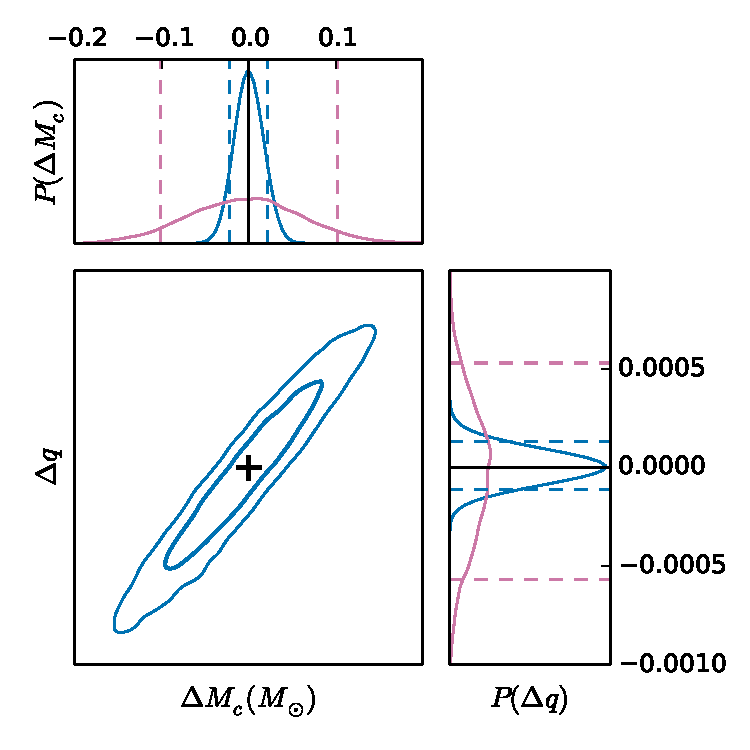
\includegraphics[width=3.4in]{figs/fig1_GR.pdf}
%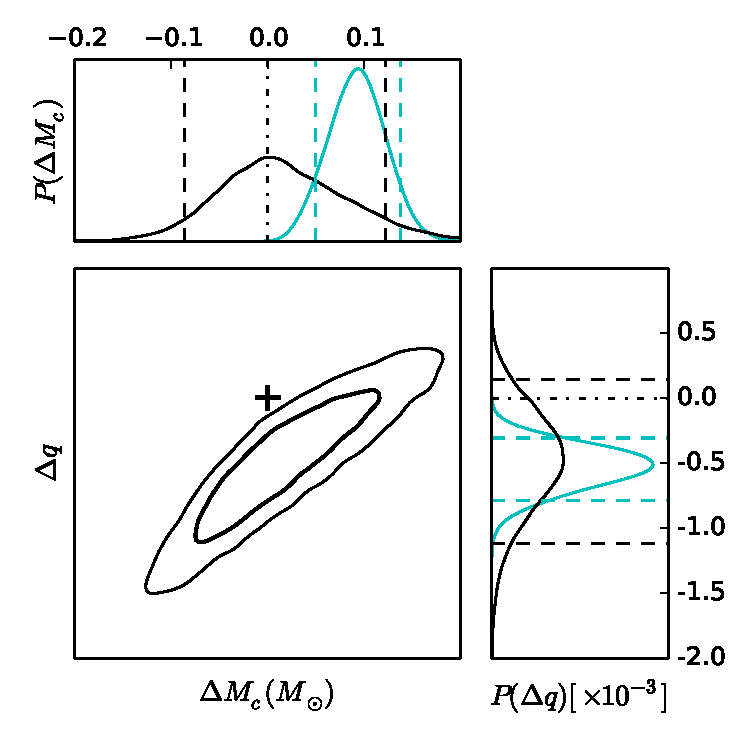
\includegraphics[width=3.4in]{figs/fig1_modGR.pdf}
\caption{The thick (thin) contours show the 68\% (95\%) credible regions in the joint posteriors of two parameters $\Delta M_c$ and $\Delta q$ that describe discrepancies in the estimated parameters using the quadrupole and non-quadrupole modes, estimated from a simulated GR signal. Black histograms on the side panels show the marginalized posteriors in $\Delta M_c$ and $\Delta q$, while the cyan histograms show the 1-dimensional posteriors in $\Delta M_c$ and $\Delta q$ estimated from the data by introducing only one variation (say, $\Delta M_c$) at a time, keeping the other fixed (say, $\Delta q = 0$). It can be seen that the posteriors are fully consistent with the GR prediction of $\Delta M_c = \Delta q = 0$ (shown by a ``+'' sign in the center panel and by thin black lines in side panels).  The simulated GR signal corresponds to a binary with total mass $M = \red{40}M_\odot$ and mass ratio $q = 9$ and an inclination angle $\iota = \red{60^\circ}$ observed by a single Advanced LIGO detector with an optimal SNR of 25. }%\emph{Right:} Same as the left plot except that the simulated signal contains a deviation from GR as described in the text. It can be seen that the posteriors are inconsistent with the GR expectation.}
\label{fig:contour_plots}
\end{center} \end{figure}
%%%%%%%%%%%%%%%%%%%%%%%%%%%%%%%%%%%%%%%%%%%%%%%%%%%%%%%%%%%%%%%%%%%%%%%%%%%%%%%%%%%%%%%%%%

Indeed, in practice it is impossible to extract different multipoles of the radiation from the GW observation of a single binary black hole system --- all we measure is a particular linear combination of multiple modes. Thus, our strategey, developed below, is to introduce extra parameters that describe inconsistency between different multipoles and to constrain those parameters using a Bayesian framework. 

The two polarizations $h_+(t)$ and $h_\times(t)$ of gravitational radiation in GR can be written as a complex time series $\h(t) := h_+(t) - i \, h_\times(t)$, which can be expanded in a basis of spin $-2$ weighted spherical harmonics~\cite{NewmanPenrose}, as:
\begin{equation}
\h(t; \n, \blambda) =  \frac{1}{d_L} \sum _{\ell=2}^{\infty} \sum _{m=-\ell}^{\ell} \Ylm (\n) \, {{\hlm}(t; \blambda)}, 
\label{eq:spherical_harmonics}
\end{equation}
where $\Ylm$ are the basis functions of spin $-2$ spherical harmonics, $\n := \{\iota, \varphi_0\}$ define the direction of radiation in the source frame, $d_L$ is  the luminosity distance to the binary, and ${\h}_{lm}(t; \blambda)$ are the spherical harmonic modes of the waveform, which are completely described by the intrinsic parameters $\blambda$ of the system. We assume that the black holes are non-spinning and the binary to be quasi-circular. Hence $\blambda$ consists of only the masses $m_1$ and $m_2$ of the black holes (it is more convenient to describe the system in terms of the \emph{chirp mass} $M_c := {(m_1m_2)^{3/5}}/{(m_1+m_2)^{1/5}}$ and mass ratio $q = m_1/m_2$). In GR, the gravitational radiation is dominated by the quadrupole modes ($\ell = 2, m = \pm 2$); however non-quadrupole modes can make an appreciable contribution if the black holes have significantly unequal masses. The set of intrinsic parameters $\blambda := \{M_c, q\}$ completely determines the multipolar structure (i.e., spherical harmonic modes) of the waveform ${\h}_{lm}(t)$. 

In order to formulate a consistency test between different multipoles, we rewrite Eq.(\ref{eq:spherical_harmonics}) by splitting the contributions from the dominant $(\ell = 2, m = \pm 2)$ mode of gravitational radiation, and the sub-dominant (higher order) modes 
\begin{eqnarray}
\h(t; \n, \blambda, \Delta \blambda) & = & \sum_{m = \pm2} Y^{-2}_{2m} (\n) {\h}_{2m}(t, \blambda)  \nonumber \\ 
& + & \sum _{\text{H.O.M}} \Ylm (\n) \hlm(t, \blambda+\Delta \blambda)
\label{eq:test_HM}
\end{eqnarray}
where the subscript H.O.M underneath the summation in the second term on the RHS indicates contribution from just the higher-order modes of the gravitational radiation. Note that we allow a possibility of inconsistency between the dominant mode and higher order modes by introducing a deviation $\Delta \blambda := \{\Delta M_c, \Delta q\}$ in the set of intrinsic parameters that describe the higher order modes; in GR,  $\Delta \blambda = 0$. 

An interferometric GW detector observes a linear combination of the two polarizations $h_+(t)$ and $h_\times(t)$, given by 
\begin{equation}
h(t) = F_+(\theta, \phi, \psi) \, h_+(t-t_0) + F_{\times}(\theta, \phi, \psi)\, {h}_{\times}(t-t_0), 
\label{eq:det_response}
\end{equation}
where $F_+$ and $F_x$ are the antenna pattern functions of the GW detector, $t_0$ is the time of arrival of the signal at the detector, and $(\theta, \phi, \psi)$ define the sky position and polarisation angle of the GW source respectively. For coalescing binary black hole (BBH) systems in quasi-circular orbits, the observed signal $h(t)$ is described by a set of \emph{intrinsic} parameters $\blambda = \{M_c, q\}$ and \emph{extrinsic} parameters  $\btheta := \{t_0, \iota, \varphi_0, d_L, \theta, \phi, \psi\}$ in GR. 
%If we consider observation using a single detector (as we do in this paper), some of the extrinsic parameters are degenerate with others, and hence it is possible to express the observed signal in terms of a smaller number of effective parameters $\btheta_\mathrm{eff} := \{t_0, \iota, \varphi_0, d_\mathrm{eff}, \psi_\mathrm{eff}\}$, where $d_\mathrm{eff} := d_L \, (F_+^2 + F_\times^2)^{-1/2}$ and $\psi_\mathrm{eff}:= \arctan (F_\times/F_+)$. 
In addition to the parameters that describe signals in GR, we introduce a set of parameters $\Delta \blambda$ describing difference between the intrinsic parameters used to generate the dominant and subdominant modes. The combined set of parameters is denoted as $\bxi = \{\blambda, \btheta, \Delta \blambda\}$. 

The data $d(t) = n(t) + h(t)$ contains the observed signal $h(t)$ given in Eq.~(\ref{eq:det_response}) along with noise $n(t)$, which is modeled as a stationary Gaussian random process 
Given data $d$ and assuming a particular model of the waveform given in \eqref{eq:test_HM} as our hypothesis $H$, it is possible to compute the posterior distribution of the set of parameters ${\bxi}$ making use of the Bayes theorem, which states: 
\begin{equation}
P({\bxi} \, | \, d, H) = \frac{P({\bxi} \, | \, H) \, P (d \, | \, {\bxi}, H)}{P(d \, | \, H)}.
\label{eq:Bayes_theorem}
\end{equation} 
The first term of the numerator on the RHS, $P({\bxi} \, | \, H)$ is the \emph{prior} distribution of the parameters ${\bxi}$, the second term $P (d \, | \, {\bxi}, H)$ is the \emph{likelihood} function, and the term in the denominator $P(d \, | \, H)$ is a normalization constant, called the \emph{evidence}. For stationary Gaussian noise with power spectral density $S_n(f)$, the likelihood can be written as:
\begin{equation}
P (d \, | \, {\bxi}, H) = \text{exp}\Big[ -\frac{1}{2}\int_{f_\mathrm{low}}^{f_\mathrm{high}} \frac{|\tilde{d}(f) - \tilde{h}(f;{\bxi}, H)|^2}{S_n(f)}df\Big]
\end{equation}
where $f_\mathrm{low}$ and $f_\mathrm{high}$ define the sensitivity bandwidth of the detector, while $\tilde{d}(f)$ and $\tilde{h}(f)$ are the Fourier transforms of $d(t)$ and $h(t)$, respectively. 

Using the above definition for the likelihood function, one proceeds to estimate $\bxi$ by stochastically sampling over the entire parameter space of interest. In this work, we use the \textsc{emcee}~\cite{goodman2010ensemble,foreman2013emcee} package, an ensemble Markhov chain Monte-Carlo (MCMC) sampler. \textsc{emcee} uses the underlying property of affine invariance of all Gaussian distributions to sample from highly skewed distributions faster than standard single-particle methods, such as Metropolis-Hastings implementations. A MCMC scheme is a random walk through the parameter space, generating samples of $\bxi$ with a probability density which ultimately converges to the stationary distribution of the Markhov chain, the posterior PDF $P(\bxi|d, H)$, using the equation of detailed balance. An \emph{ensemble} MCMC sampler implements a coordinated random walk of multiple ``walkers" through the parameter space, such that each step of the Markhov chain, or updating the position of any one walker at a particular time step, is influenced by the positions of the rest of the walkers. The algorithm requires the hand-tuning of a small set of 1-2 parameters, and can be easily parallelized to use multiple computing cores, giving it major advantages over traditional MCMC algorithms~\footnote{We have compared the posterior distributions obtained from our \textsc{emcee} based code with that from the Nested-Sampling based \textsc{LALInferenceNest} code~\cite{Veitch:2009hd} that is employed for Bayesian parameter estimation in LIGO-Virgo scientific collaboration. Posteriors obtained from simulated GR waveforms containing only the dominant ($\ell = 2, m = \pm 2$) modes observed by a single detector are in good agreement.}. From the posterior distribution $P(\bxi | d, H)$ of the full parameter set, we construct the posterior distribution $P(\Delta \blambda | d, H)$ of the set of parameters describing deviation from GR prediction, by marginalizing the posterior over all other parameters $\{\blambda, \btheta\}$. If the data is consistent with GR, we expect $P(\Delta \blambda | d, H)$ to be consistent with zero. 

\paragraph{Simulations using GR waveforms:---}
Here we demonstrate this test making use of simulated GW observations from binary black holes where the waveforms are modelled after the GR prediction. We employ the recent inspiral-merger-ringdown waveform model proposed by Mehta \etal~\cite{Mehta:2017jpq}, which provide accurate Fourier-domain models of the following spherical harmonic modes $\h_{\ell m}(f)$ of the expected GW signals from non-spinning binary black holes: $(\ell = 2, m = \pm2)$, $(\ell = 2, m=\pm1)$, $(\ell = 3, m=\pm3)$, $(\ell = 4, m = \pm4)$. (The other spherical harmonic modes that are neglected only introduce an inaccuracy (mismatch) of less than 1\% in the waveforms~\cite{Mehta:2017jpq}). GW observations are simulated by combining these signals with stationary Gaussian noise with power spectral density anticipated in Advanced LIGO's ``high-power, zero-detuning'' configuration~\cite{aLIGOZeroDetHighPower} making use of Eqs.~(\ref{eq:spherical_harmonics}) and (\ref{eq:det_response}). We consider binaries with total mass $M := m_1 + m_2$ in the range $20 M_\odot$ -- 200 $M_\odot$ with mass ratio $q := m_1/m_2$ in the range 1 -- 9, with varying inclination angles $\iota$ (angle between the orbital angular momentum of the binary and the line of sight). 

We perform the test by introducing variations in the higher order modes: The higher-order modes $\hlm(f; \blambda+\Delta\blambda)$ are generated by introducing an extra parameter $\Delta\blambda$ while the quadrupole-modes $\h_{2\pm2}(f; \blambda)$ are generated by using the standard set of parameters $\blambda$ in GR. We have experimented with different choices for the deviation parameter $\Delta\blambda$: 
\begin{enumerate}
\item By introducing \emph{one} deviation parameter at a time. That is, $\Delta\blambda = {\Delta M_c}$ or $\Delta\blambda = {\Delta q}$. 
\item By introducing a concurrent deviation in \emph{two} parameters $\Delta \blambda = \{\Delta M_c, \Delta q\}$. 
\end{enumerate}
We show in Fig.~\ref{fig:contour_plots} the results of the tests performed by varying either one parameter or two parameters, for the system with total mass $M = 80M_{\odot}$, mass ratio $q=9$, inclination angle $ {\iota}=60^{\circ} $ producing a signal-to-noise ratio  (SNR)  of 25 (SNR in higher modes is $\sim 10$). It can be seen that the results are consistent with the expected value in GR. As expected, the width of the posteriors are smaller when only one variation is introduced at a time. Figures~\ref{fig:dMc_dq_posteriors_gr_vs_q} and \ref{fig:dMc_dq_posteriors_gr_vs_M} show the expected width of the 90\% credible regions of the posteriors of the parameters describing deviations from GR, for the case of binaries with different masses, mass ratios and inclination angles. For all cases, the SNR of the injections is set to \red{25}.  It is clear that binaries with large mass ratios ($q > 2$) in inclined orbts ($\iota > 60 ^\circ $) will allow precision tests of the GR predictions, reaching statistical uncertainties of $<  10^{-2}$ for $\Delta M_c/Mc$ and $\Delta q$.   

\begin{figure}[tbh]
	\includegraphics*[width=3.5in]{figs/fig3.pdf}
	\caption{The figure shows the width of the 90$\%$ credible region of $\Delta M_c$ and $\Delta q$ for binaries with different mass ratios $q$ (horizontal axis) and inclination angles $\iota$ (legends). All binaries have a total mass $40M_{\odot}$. Best constraints are provided by binaries with high mass ratios and/or large inclination angles.}
	\label{fig:dMc_dq_posteriors_gr_vs_q}
\end{figure}

\begin{figure}[tbh]
	\includegraphics*[width=3.5in]{figs/fig3b.pdf}
	\caption{Same as Fig.~\ref{fig:dMc_dq_posteriors_gr_vs_q}, except that the horizontal axis reports the total mass $M$. All binaries correspond to a mass ratio $q = 9$.}
	\label{fig:dMc_dq_posteriors_gr_vs_M}
\end{figure}


% \paragraph{Simulations using modified-GR waveforms:---}
% 
% We also investigate the efficacy of our test in detecting deviations from GR. We introduce a deviation from GR in the simulated signals --- a propagation effect predicted by the Chern-Simons (CS) gravity. Under the CS modification to GR, a circularly polarized plane GW, propagating on an Friedmann–Lema\^itre–Robertson–Walker spacetime, would show amplitude birefringence and parity violation~\cite{Yunes:2010yf}. Compared to GR, right circularly polarized waves will be exponentially enhanced or suppressed with respect to left circularly polarized waves, as they propagate. That is, 
% % 
% \begin{equation}
% \h_\mathrm{R,L}^\mathrm{mod} = \h_\mathrm{R,L} \, e^{-i \, \delta\phi_\mathrm{R,L}} \simeq  \h_\mathrm{R,L} \, (1 \mp i \, \delta\phi),
% \label{eq:cs_modification_h}
% \end{equation}
% where $\h_\mathrm{R,L} = (h_+ \pm i \, h_\times)/\sqrt{2}$ are the right/left circularly polarized polarization states predicted by GR and $\delta \phi$ is an additional phase contribution due to the CS correction, given by 
% \begin{equation}
% \delta \phi = i \, f \, \pi \, z \, \Big(\dot{\theta_0}-\frac{\ddot{\theta_0}}{H_0}\Big).
% \label{eq:cs_modification_dphi}
% \end{equation}
% Here, $f$ is the Fourier frequency measured by the observer, $z$ is the cosmological redshift at source, and ${H_0}$ is the value of the Hubble constant measured by the observer, while $\dot{\theta_0}$ and $\ddot{\theta_0}$ denote the first and second time-derivative of the CS coupling field. Note that the CS correction is purely imaginary which results in amplitude birefringence. Solar system observations of the LAGEOS satellites have allowed us to derive a bound $|\dot{\theta_0}-\frac{\ddot{\theta_0}}{H_0}| < 2000~\mathrm{km}$~\cite{Yunes:2010yf,Smith:2007jm}.
% 
% From the $+,\times$ polarizations of the GR waveforms discussed in the earlier section, we construct a modified-GR waveforms by introducing the propagation effects described in Eq.\eqref{eq:cs_modification_h}, with $\dot{\theta_0}-\frac{\ddot{\theta_0}}{H_0} = 2000~\mathrm{km}$. Example of such a modified waveform is shown in Fig.~\ref{fig:mod_gr_waveform} for a system $M = 80M_{\odot}$, $q =9$, $\iota = 90^{\circ}$,solar system constraint at a distance of 200Mpc. We inject this waveform into simulated noise and perform the Bayesian parameter estimation described earlier. The resulting injected waveform has an optimal SNR of \red{XXX} in the detector, of which \red{$\sim XX\%$} is distributed in the non-quadrupole modes. Figure~\ref{fig:contour_plots} (right panel) shows the posteriors on parameters describing describing deviations from the GR prediction. It can be seen that the posteriors on deviation parameters $\{\Delta M_c, \Delta q\}$ are inconsistent with the GR prediction, $\{0, 0\}$. 
% 
% \begin{figure}[h]
% 	\includegraphics*[width=3.1in]{figs/mod_GR_waveform.pdf}
% 	\caption{Fourier-domain amplitudes of GR and modified GR waveform with the modification $\delta \phi_\mathrm{R,L} = \pm i \, 10^{-3} f$ [see, Eq.\eqref{eq:cs_modification_dphi}]. The system configuration is $M = 80 M_{\odot}$, $q = 9$, $\iota=60^{\circ}$ at a distance of 400 Mpc. The match between GR and modified-GR waveform is greater than \red{XX}.}
% \label{fig:mod_gr_waveform}
% \end{figure}


\begin{figure}[tbh]
	\includegraphics*[width=3.5in]{figs/q_and_iota_dist.pdf}
	\caption{Cumulative distribution of the mass ratio $q$ (left) and inclination angle $\iota$ of simulated binary black holes that are detectable by Advanced LIGO. The two distributions in the left plot corresponds to two assumed distributions of the component masses (see text).}
	\label{fig:q_iota_distribution}
\end{figure}


\paragraph{Astrophysical prospects:---}  Note that, this test requires the observation of GW signals where the subdominant modes can be observed with appreciable SNR. These modes are excited predominantly for binaries with large mass ratios. Also, due to the radiation pattern, radiation from binaries with highly inclined orbits will contain appreciable contribution from subdominant modes. Hence binaries with large mass ratios ($q \gtrsim 2$) and inclined orientations ($\iota \gtrsim 60^{\circ}$) are particularly suitable sources for permorming the test described in this paper. This test can not be performed on the GW signals observed by LIGO and Virgo during their first two observational runs, for which mass ratios are close to 1 and inclinations are closed to face-on ($\iota \sim 0$). Detection rates of binaries with large mass ratios depend on the astrophysical merger rates of such binaries, which is currently uncertain, while the detection rate of binaries with large inclination angle is related to the same with small inclination angles by a simple geometric factor. 

Here we investigate the  prospects of performing such a test on binary black hole events that  Advanced LIGO expects to observe over the new few years.  We simulate populations of binary black holes based on reasonable astrophysical assumptions, and examine the distributions of the mass ratio and inclination angle of detectable signals. In particular, we simulate binaries with two assumed distributions of component masses in the source-frame~\cite{Abbott:2016nhf}:
\begin{enumerate}
\item Masses flat in $\log m_1$ and $\log m_2$   with $5 M_\odot \leq m_1, m_2  \leq 100 M_\odot$. 
\item Masses following a power-law $p(m_1) = m_1^{-2.35}$ on the mass of the larger black hole, with the smaller mass distributed uniformly in $q$ and with $5 M_\odot \leq m_1, m_2  \leq 100 M_\odot$. 
\end{enumerate}
In both cases, binaries are distributed uniformly in the sky with isotropic orientations. The distribution of the mergers in redshift is chosen according to the prescription given in~\cite{Dominik:2013tma}. The cosmoligcal redshift on the GW signals can be absorbed by a rescaling of the masses $m_{1,2} (1+z)$ where $z$ is the redshift. From the simulated events, we compute the SNR expected  in Advanced LIGO and apply an SNR threshold for detection (the probability distributions are independent of the exact value of the SNR threshold). The cumulative distribution of the mass ratio $q$ and inclination angle $\iota$ of binaries crossing the detection threshold is plotted in Fig.~\ref{fig:q_iota_distribution}. It can be seen that $\sim 20 - 40\%$ of the detectable binaries will have a mass ratio greater than 2, out of which  $\sim 15\%$ will  be observed with inclination angle greater than $60^\circ$. This suggests that only a few percent of the observed binaries are likely to have large mass ratios ($q > 2$) and inclined orbits ($\iota > 60^\circ$). However, since Advanced LIGO and Virgo are expected to observe hundreds of binary black hole events over the next few years~\cite{Abbott:2016nhf}, we expect that a handful of signals will be detected using with this test can be performed. 

\paragraph{Conclusions and future work:---} In this paper, we proposed a new method to test the consistency of an observed GW signal with a binary black hole system predicted by GR. The test relies on the fact that, given the parameters of a binary black hole system, the multipolar structure of the radiated GW signal is uniquely predicted by GR. Thus, if we estimate the parameters of the binary from different spherical harmonic modes of the observed signal independently, those estimates have to be consistent with each other. Any inconsistency between the different estimates will point to a deviation from GR or to the non-black hole nature of the compact objects in the binary. We developed a Bayesian parameter estimation method to identify potential deviations from GR predictions and tested this method using simulated GW signals.  We provided the first estimates of the expected precision of such tests that can be performed using GW observations of binary black holes anticipated by Advanced LIGO and Virgo in the next few years. 

Note that in this paper we assume, for simplicity, that the black holes in the binary have negligible spins. However, the method can be easily generalized to the case of binaries consisting of spinning black holes. Indeed, the systematic errors due to inaccuracies in the waveform modeling and detector calibration errors need to be understood before implementing such a test on real observations. We leave these as future work. 

\paragraph{Acknowledgments:---}
We thank Chandra Kant Mishra for help with the numerical implementation of the waveform model used in this paper and K. Haris for help with the astrophysical simulations. This research was supported by the Indo-US Centre for the Exploration of Extreme Gravity funded by the Indo-US Science and Technology Forum (IUSSTF/JC-029/2016). P.~A.'s research was, in addition, supported by a Ramanujan Fellowship from the Science and Engineering Research Board, India and by the Max Planck Society through a Max Planck Partner Group at ICTS-TIFR. Computations were performed at the ICTS cluster Alice. 
%
\bibliographystyle{apsrev-nourl}
\bibliography{TGR_HM}

\end{document}
